\documentclass{beamer}
\usepackage{amsfonts,amsmath,oldgerm}

\usepackage[utf8]{inputenc}
\usepackage[T1]{fontenc}
\usepackage{graphicx}
\usepackage{listings}
\usepackage{hyperref}
\usepackage{verbatim}
\usepackage{siunitx}
\usepackage{bm}

\usepackage[english]{babel}
\usepackage[export]{adjustbox}
\usepackage{caption} %For subfigures
\usepackage{subcaption} %For subfigures
\usepackage{placeins} %FloatBarriers

\usetheme{sintef}

\newcommand{\testcolor}[1]{\colorbox{#1}{\textcolor{#1}{test}}~\texttt{#1}}

\usefonttheme[onlymath]{serif}
\graphicspath{{assets/images/}}


\titlebackground*{assets/logos/background}

\newcommand{\hrefcol}[2]{\textcolor{cyan}{\href{#1}{#2}}}

\title{Numerical study of the airflow over a high-altitude pseudo-satellite wing}
\subtitle{PhD update}

\author{\href{mailto:mail@carlobrunelli.com}{Carlo Brunelli}}


\newcommand{\VV}[1] {\vv{\vv{#1}}}

\begin{document}
\maketitle


\begin{frame}

PhD presentation after 1.5 years
\begin{itemize}
	\item \textit{Is it possible to implement efficiently the Variational Multiscale Method in the Julia programming language?}
	\item \textit{Is it suitable to study transitional airfoils at low-Reynolds?}
\end{itemize}

\begin{figure}[h]
	\centering          
		\includegraphics[width=0.55\textwidth]{ du89_vcontour.png}
		\caption{DU89 velocity contour, $u_z$ colormap}
	\end{figure} 
\end{frame}

\section{Numerical Methods}
\begin{frame}{Numerical Method implemented}
The numerical method currently implemented are:
  \begin{itemize}
    \item Variational Multiscale Method (VMS)
    \item Streamline upwind Petrov–Galerkin (SUPG)
  \end{itemize} 

Different solution method are available for all of them 
  \begin{itemize}
    \item Non-linear (NLIN)
    \item Linearized-Coupled (LC-VMS)
    \item Linearized-Segregated (LS-VMS)
  \end{itemize} 
\end{frame}


\begin{frame}{Variational Multiscale Method}
  \begin{itemize}
    \item Evolution of the SUPG
    \item Implict LES
    \item It does not need calibration
    \item Residual-based stabilization
  \end{itemize} 
\end{frame}


\begin{frame}{Galkerkin formulation}
Conservation of mass:
\begin{equation}
    \nabla\cdot \Vec{u} = 0
    \label{equfo:cont}
\end{equation}

Conservation of momentum:
\begin{equation}
    \dfrac{\partial \Vec{u}}{\partial t} + (\Vec{u}\cdot\nabla)\Vec{u} + \nabla p - \nu\Delta\Vec{u} - f = 0
        \label{equfo:mom}
\end{equation}

Variational Formulation
\begin{equation}
\begin{split}
  B^G = &   \int_\Omega \dfrac{\partial \Vec{u}}{\partial t}\cdot \Vec{v}\;d\Omega +
    \int_\Omega(\Vec{u}\cdot\nabla)\Vec{u}\cdot \Vec{v} \;d\Omega+ 
    \int_\Omega \nabla (p)\cdot\Vec{v} \;d\Omega + \\
     & \int_\Omega\nu\nabla\Vec{u}\cdot\nabla\Vec{v} \;d\Omega  -
        \int_\Omega f\cdot\Vec{v} \;d\Omega + 
    \int_\Omega q(\nabla \cdot \Vec{u})\;d\Omega = 0
    \end{split}
    \label{equ:weak}
\end{equation}

\end{frame}

\begin{frame}{Stabilization equations}
\begin{equation}
B^{SUPG}(t, (\Vec{u},p), (\Vec{v},q))  =     \int_\Omega(\tau_m(\Vec{u}\cdot\nabla \Vec{v} +\nabla q)\cdot\Vec{R_m} \;d\Omega+ \int_\Omega \tau_c (\nabla \cdot \Vec{v})R_c \;d\Omega
\label{equ:bsupg}
\end{equation}

\begin{equation}
B^{VMS1}(t, (\Vec{u},p), (\Vec{v},q))  = \int_\Omega (\Vec{u}\cdot\nabla \Vec{v}')\odot(\tau_m \Vec{R_m}) \;d\Omega
\label{equ:bvms1}
\end{equation}


\begin{equation}
B^{VMS2}(t, (\Vec{u},p), (\Vec{v},q))  = -\int_\Omega (\nabla\Vec{v}\odot(\tau_m \Vec{R_m} \otimes \tau_m \Vec{R_m}) \;d\Omega
\label{equ:bvms2}
\end{equation}

\end{frame}


\begin{frame}{Stabilization parameters}

\begin{equation}
\tau_m =\bigg( \dfrac{4}{\Delta t^2} + \Vec{u}\cdot{G}\Vec{u} + C_I \nu^2 {G}:{G} \bigg)^{-1/2}
\label{equ:taum}
\end{equation}

\begin{equation}
\tau_c = (\tau_c\Vec{g}\cdot\Vec{g})^{-1}
\label{equ:tauc}
\end{equation}

Where G is the inverse of the gradient of the map cell.
For a cubed shaped element, with $h$ the edge length, $G_{ij} =\dfrac{1}{h^2}\delta_{ij}$, where $\delta_{ij}$ is the Kronecker delta.

\end{frame}


\begin{frame}{Linearization}

\begin{equation}
    \tilde{\Vec{u}} = 2.1875 u^{n} - 2.1875 u^{n-1} + 1.3125 u^{n-2} - 0.3125 u^{n-3} 
    \label{equlin:taylor_exp}
\end{equation}

\begin{equation}
 (\Vec{u}\cdot\nabla)\Vec{u} \Rightarrow  (\tilde{\Vec{u}} \cdot\nabla)\Vec{u} 
\end{equation}


\end{frame}






\section{Performances}
\begin{frame}{Weak Scaling}
Weak scalability: the solution time almost does not change with constant problem size per processor
\begin{figure}
         \centering
         \includegraphics[width=0.5\textwidth]{TaylorGreen_Weak_Scalability_VMS_lin_nlin.pdf}
         \caption{Taylor Green weak scalability}
\end{figure} 
\end{frame}

\begin{frame}{Strong Scaling}
Strong scalability: doubling the number of processors halves the solution time

\begin{figure}
         \centering
         \includegraphics[width=0.5\textwidth]{TaylorGreen_Strong_Scalability_VMS_lin_nlin.pdf}
         \caption{Taylor Green Strong scalability}
\end{figure} 
\end{frame}

\section{Boundary Layer Initialization}
\begin{frame}{Boundary Layer Initialization}
    \begin{itemize}
    \item Avoid Instabilities (close to the leading edge)
    \item Avoid velocity ramping
    \item Allows Higher time-step
    \end{itemize}


    \begin{figure}[h]
        \centering          
        \begin{subfigure}[h]{0.45\textwidth}
                 \centering
            \includegraphics[width=\textwidth]{mesh_du89.png}
       \end{subfigure}
             \hfill
        \begin{subfigure}[h]{0.45\textwidth}
         \centering
            \includegraphics[width=\textwidth]{mesh_du89_le.png}
        \end{subfigure}
        \caption{Mesh DU89}
        \end{figure} 
\end{frame}



\begin{frame}{Find wall-distance}

    Using the function exploited by RANS solvers for the wall distance for computing turbulent parameters but now used to detect the airfoil's contour
    \begin{equation}
    \begin{cases}
        \nabla \cdot (|\nabla u_p|^{p-2} \nabla u_p) = -1 & x\in \Omega\\
        u_p = 0 & x\in \Omega_D
        \end{cases}
        \label{equ:ppoisson}
    \end{equation}
    The true-wall distance is provided by solving the equation for $p\xrightarrow{}\infty$
    Solved using a method that resembles Picard's
    \end{frame}
    

    \begin{frame}{Find wall-distance}
    \begin{equation}
        v_p = -|\nabla u_p|^{p-1} + \bigg ( \dfrac{p}{p-1}u_p +  |\nabla u_p|^{p}\bigg ) ^{\dfrac{p}{p-1}}
        \label{equ:vpoisson}
    \end{equation}
    \begin{enumerate}
        \item It starts solving the equation for p=2
        \item \begin{equation}
            \int \bigg (\nabla (v) \cdot (\nabla u_{hp}) \bigg )d\Omega = \int \bigg( 1\cdot v \bigg )d\Omega
        \end{equation}
        \item It solves the linearized equation, which becomes \eqref{equ:ppoisson-fem2}. In this case solving for p=3 the $\tilde{u}$ is $uh_2$
          \begin{equation}
            \int \bigg (\nabla (v) \cdot (|\nabla \tilde{u}|^{p-2} \nabla u) \bigg )d\Omega = \int \bigg( 1\cdot v \bigg )d\Omega
            \label{equ:ppoisson-fem2}
        \end{equation}
        \item It is not possible to iterate step 3 for p > 3, the solution becomes unstable. It introduces the relaxation coefficient $\gamma = 0.5$ and it starts an internal cycle.
    \end{enumerate}
    \end{frame}

    \begin{frame}{Boundary Layer Initialization}
    The velocity in the $x$ direction in the region identified can be with a simple cubic function \eqref{equ:bl-cubic-init} where $dn = d/\delta_{99}$, $d$ is the minimum distance to the airfoil, $u_\infty$ is the free-stream flow speed.
    \begin{equation}
        f(dn) = 
        \begin{cases}
            u_\infty & dn>1\\
            ( -dn^2+2\cdot dn )\cdot u_\infty &  dn<1
        \end{cases}
        \label{equ:bl-cubic-init}
    \end{equation}
     The boundary layer function has been obtained by fixing the following boundary conditions:
    \begin{itemize}
        \item Continuity with the external flow, $f(1)=1$ 
        \item Smooth transition between boundary layer and external flow, $f'(1)=0$ 
        \item Non-slip condition at the wall, $f(0)=0$
    \end{itemize}
    \end{frame}
    
    \begin{frame}{Boundary Layer Initialization}
    It results in a low-speed zone close to the airfoil, avoiding high speed in really small cells useful for capturing the boundary layer.
    \begin{figure}
             \centering
             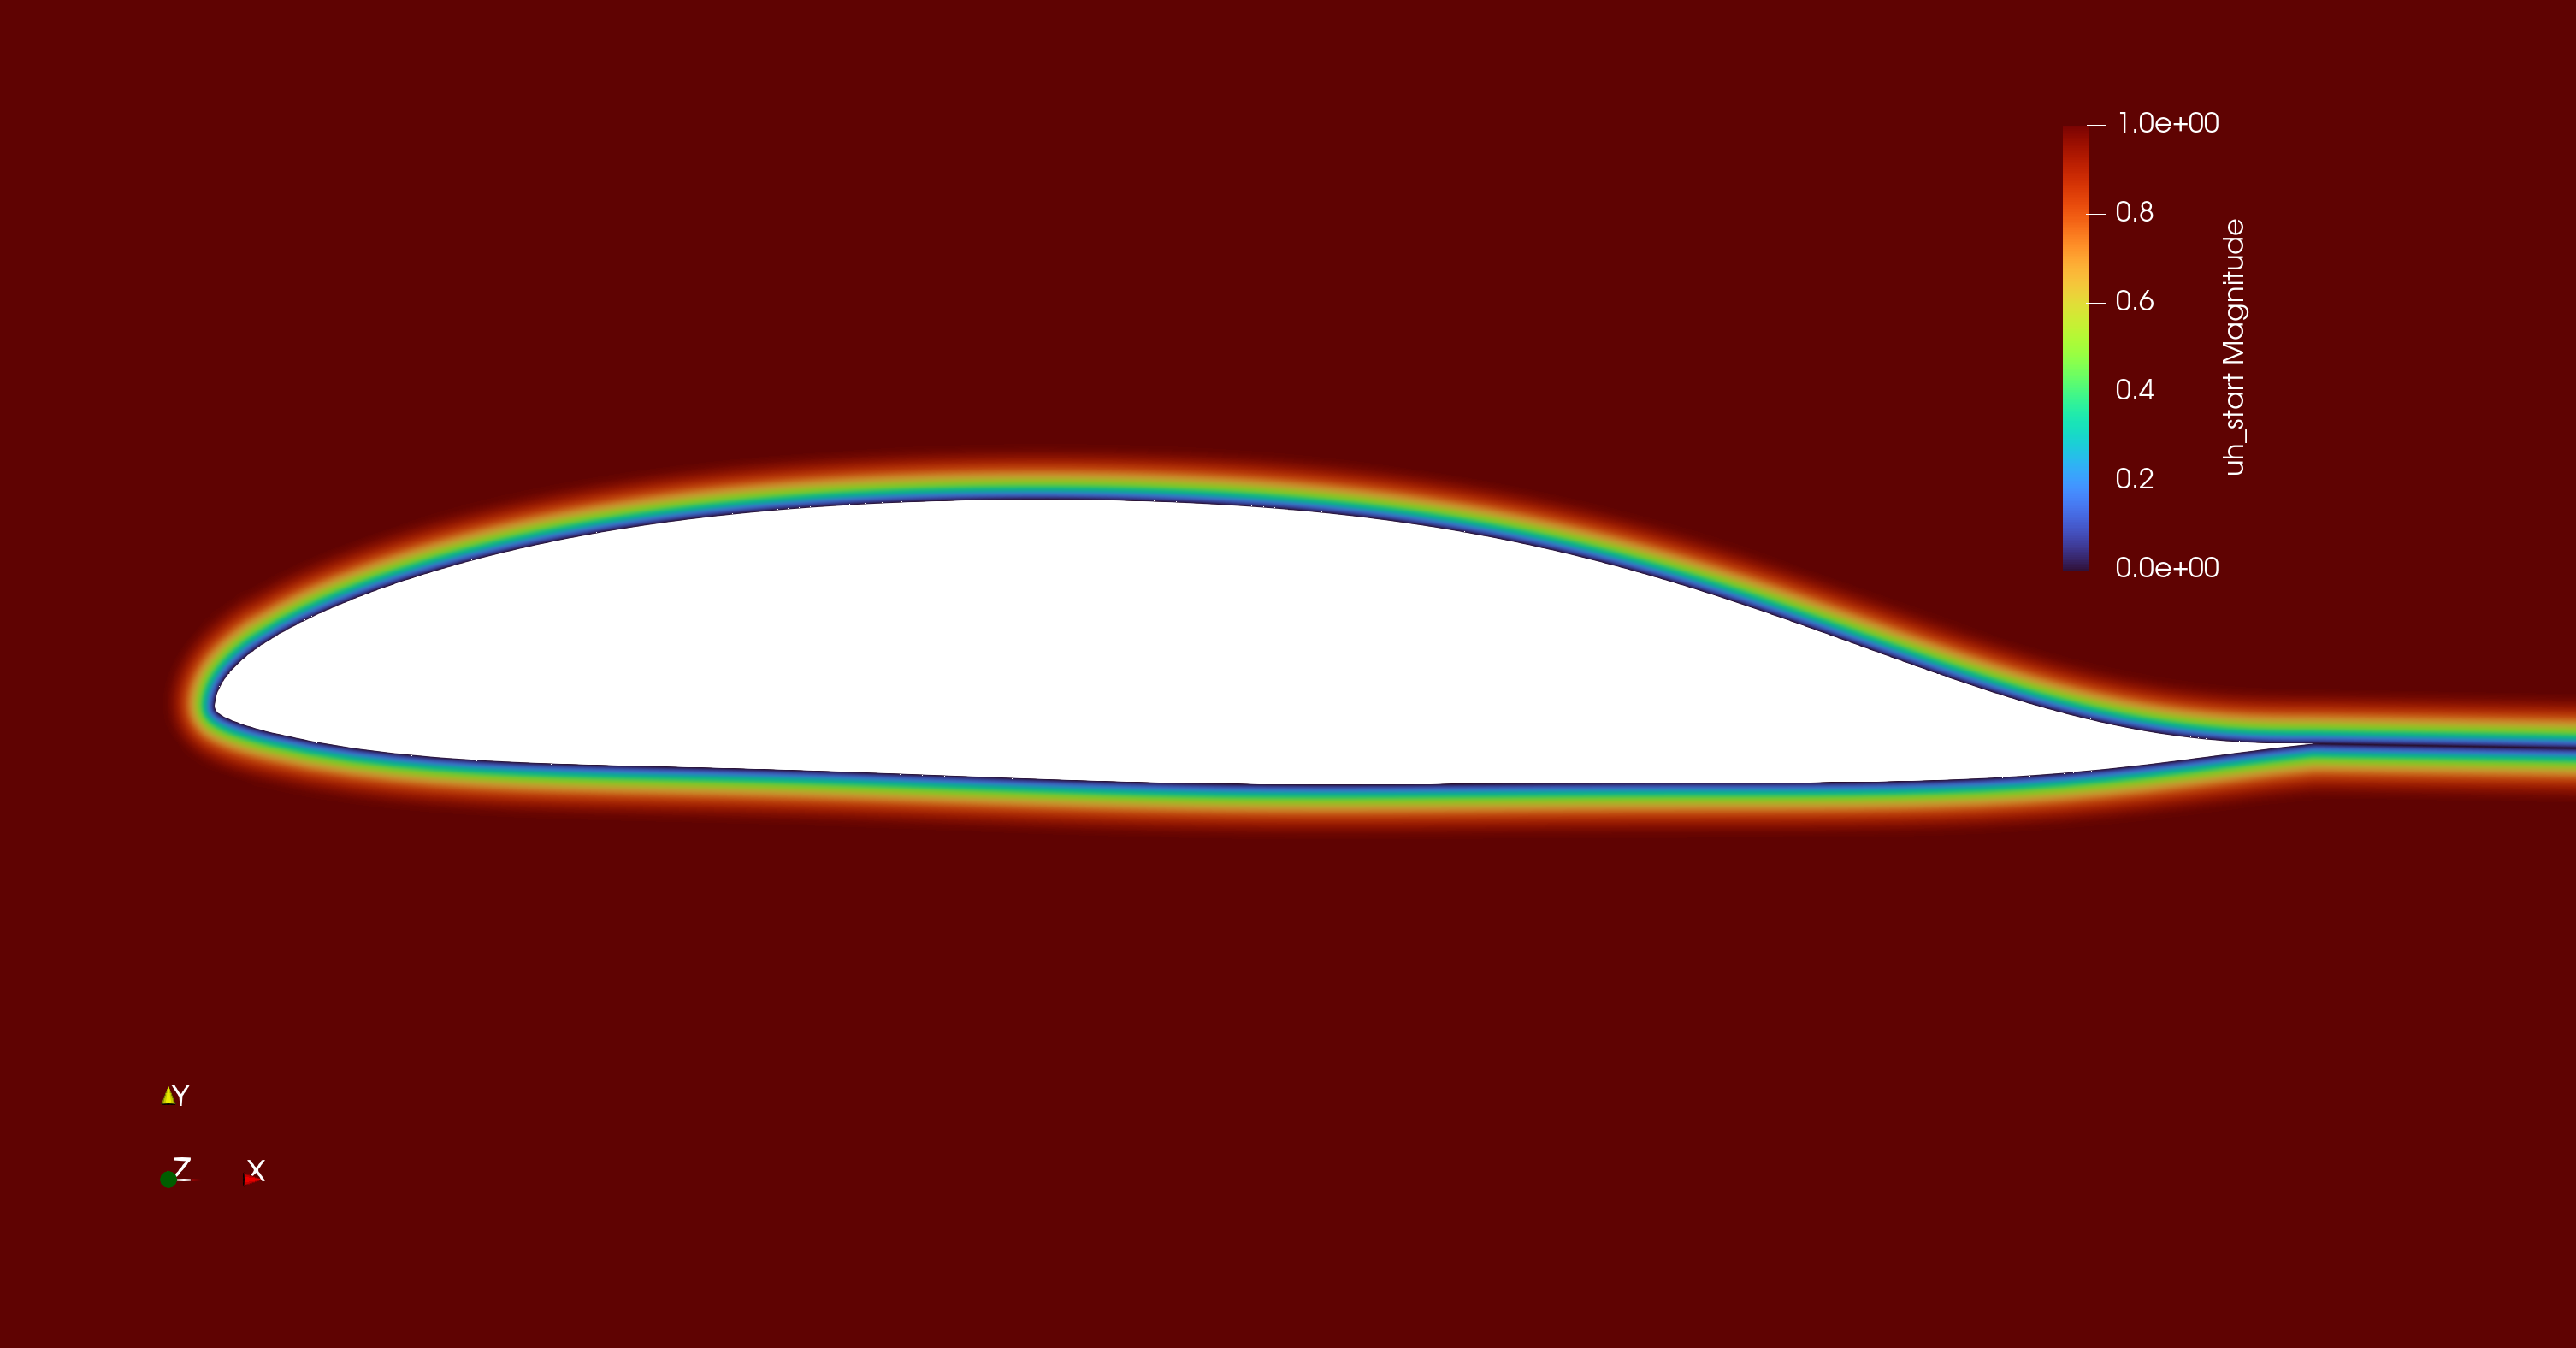
\includegraphics[width=0.65\textwidth]{WallDistanceDU89.png}
             \caption{Boundary Layer Initialization}
             \label{fig:wall-distance-init}
    \end{figure} 
    \end{frame}
    

\section{Synthetic Eddy Method}
\begin{frame}{SyntheticEddyMethod.jl}
\begin{itemize}
\item \href{https://www.theoj.org/joss-papers/joss.05565/10.21105.joss.05565.pdf}{publication}
\item presented at \textit{JuliaCon2023} at MIT
\end{itemize}

Features:
\begin{itemize}
\item Create fluctuations that respect the divergence-free condition (DFSEM)
\item Create velocity fluctuations for inlet boundary conditions
\item Create coherent eddies in 3D domain
\item Define custom Reynolds Stress Tensor
\item Import from file custom Reynolds Stress Tensor
\end{itemize}
\end{frame}


\begin{frame}{Synthetic Eddy Method}
Reynolds decomposition:
\begin{equation}
    \Vec{u}(\Vec{x},t) = \Vec{U}(\Vec{x},t) +  \Vec{u'}(\Vec{x},t)
    \label{sem:u}
\end{equation}

Compute velocity fluctuations, using a suitable shape function:
\begin{equation}
u_i(\boldsymbol{x})=U_i(\boldsymbol{x})+\frac{1}{\sqrt{N}} \sum_{k=1}^N a_{i j} \epsilon_j^k f_{\sigma(\boldsymbol{x})}\left(\boldsymbol{x}-\boldsymbol{x}^k\right)
\label{sem:ui}
\end{equation}
\end{frame}


\section{Laminar Separation Bubble}




\begin{frame}{Simulations}
\begin{itemize}
\item VMS linearized coupled sd7003s - Re $\num{60000}$ - AoA $\ang{4}$ 
\item VMS linearized segregated DU89 - Re $\num{250000}-\num{500000}$ - AoA $\ang{1}-\ang{5}$ 
\end{itemize}
\end{frame}

\begin{frame}{Models}
sd7003s - Re $\num{60000}$ - AoA $\ang{4}$ 
\begin{figure}[h]
     \centering          
         \includegraphics[width=0.65\textwidth]{ sd7003_differentmodels.pdf}
         \caption{Different model provides different results. RANs use $\gamma -Re_ \theta$ model.}
     \end{figure} 
\end{frame}

\begin{frame}{VMS linearized coupled sd7003s}
Copuled: velocity and pressure are solved at the same time.
Re $\num{60000}$ - AoA $\ang{4}$ . Initialization with velocity-ramping
\begin{figure}[h]
     \centering          
     \begin{subfigure}[h]{0.45\textwidth}
              \centering
         \includegraphics[width=\textwidth]{sd7003_cf.pdf}
    \end{subfigure}
          \hfill
     \begin{subfigure}[h]{0.45\textwidth}
      \centering
         \includegraphics[width=\textwidth]{sd7003_cp.pdf}
     \end{subfigure}
\caption{Comparison with VMS literature results}
     \end{figure} 
     
\end{frame}

\begin{frame}{ VMS linearized coupled sd7003s}
\begin{figure}[h]
     \centering          
         \includegraphics[width=0.8\textwidth]{SD7003_Cf_zoom.pdf}
         \caption{Bubble position function of freestream turbulence intensity}
     \end{figure} 
\end{frame}




\begin{frame}{VMS Linearized-Segregated}
Segregated: each time step pressure and velocity system are solved one after the other multiple times. It is possible to re-use the matrices and preconditioner. It is an iterative method.

\end{frame}




\begin{frame}{VMS Linearized-Segregated}
PhD research aims to simulate new a new airfoil.
Re $\num{250000}$ - AoA $\ang{1}$ 

\begin{figure}[h]
     \centering          
     \begin{subfigure}[h]{0.45\textwidth}
              \centering
         \includegraphics[width=\textwidth]{DU89_250000_AoA_1_Cf.pdf}
    \end{subfigure}
          \hfill
     \begin{subfigure}[h]{0.45\textwidth}
      \centering
         \includegraphics[width=\textwidth]{DU89_250000_AoA_1_Cp.pdf}
     \end{subfigure}
     \end{figure} 
 \end{frame}

\begin{frame}{VMS Linearized-Segregated}
Re $\num{250000}$ - AoA $\ang{5}$ 
\begin{figure}[h]
     \centering          
     \begin{subfigure}[h]{0.45\textwidth}
              \centering
         \includegraphics[width=\textwidth]{DU89_250000_AoA_5_Cf.pdf}
    \end{subfigure}
          \hfill
     \begin{subfigure}[h]{0.45\textwidth}
      \centering
         \includegraphics[width=\textwidth]{DU89_250000_AoA_5_Cp.pdf}
     \end{subfigure}
     \end{figure} 
 \end{frame}

\begin{frame}{VMS Linearized-Segregated}
Re $\num{500000}$ - AoA $\ang{1}$ 
\begin{figure}[h]
     \centering          
     \begin{subfigure}[h]{0.45\textwidth}
              \centering
         \includegraphics[width=\textwidth]{DU89_500000_AoA_1_Cf.pdf}
    \end{subfigure}
          \hfill
     \begin{subfigure}[h]{0.45\textwidth}
      \centering
         \includegraphics[width=\textwidth]{DU89_500000_AoA_1_Cp.pdf}
     \end{subfigure}
     \end{figure} 
 \end{frame}

\begin{frame}{VMS Linearized-Segregated}
Re $\num{500000}$ - AoA $\ang{5}$ 
\begin{figure}[h]
     \centering          
     \begin{subfigure}[h]{0.45\textwidth}
              \centering
         \includegraphics[width=\textwidth]{DU89_500000_AoA_5_Cf.pdf}
    \end{subfigure}
          \hfill
     \begin{subfigure}[h]{0.45\textwidth}
      \centering
         \includegraphics[width=\textwidth]{DU89_500000_AoA_5_Cp.pdf}
     \end{subfigure}
     \end{figure} 
 \end{frame}



\section{Uncertainty Quantification}
\begin{frame}{Model Variables}
\begin{itemize}
    \item    TI - turbulence intensity
    \item $\mu r$ - turbulent viscoity ratio
\end{itemize}

$k-\omega$ parameters:
\begin{itemize}
    \item $\sigma \omega 1$
    \item $\alpha 1$ 
    \item $\beta *$  
\end{itemize}
$\gamma Re_\theta$ parameters
\begin{itemize}
\item $s1 $
\item $C1$
\end{itemize}
\end{frame}


\begin{frame}{Sobolov Indexes}
    \begin{figure}
        \centering
        \includegraphics[width=0.7\textwidth]{Sobol_Indexes_sd7003.pdf}
        \caption{Sobol' indices for 3D RANS variables}
\end{figure} 
\end{frame}

\section{Conclusions}
\begin{frame}{Other activities}
    \begin{itemize}
        \item Synthetic Eddy Method \href{https://www.theoj.org/joss-papers/joss.05565/10.21105.joss.05565.pdf}{publication}
        \item JuliaCon 2023 conference
        \item Co-author AIAA 2023 conference paper
    \end{itemize}
    
    \begin{itemize}
        \item Testing standard passive flow controls (no improvement in aerodynamic efficiency)
    \end{itemize}
    \begin{figure}[h]
        \centering          
        \begin{subfigure}[h]{0.30\textwidth}
                 \centering
            \includegraphics[width=\textwidth]{Slot.pdf}
            \caption{Slot}
       \end{subfigure}
       \hfill	
       \begin{subfigure}[h]{0.30\textwidth}
                \centering
           \includegraphics[width=\textwidth]{Slot-curved.pdf}
           \caption{Slot curved}
        \end{subfigure}
             \hfill
        \begin{subfigure}[h]{0.30\textwidth}
         \centering
            \includegraphics[width=\textwidth]{Riblet.pdf}
            \caption{Riblet}
        \end{subfigure}
        \caption{Passive Flow Controls}
        \end{figure} 
    \end{frame}
    
    
    
    \begin{frame}{Elements of novelty}
    \begin{itemize}
        \item Systematic usage of Julia in fluid-dynamics
        \item Usage of VMS for high Reynolds airfoil
        \item First LES code in Julia - fully parallelized - working with 3D airfoils up to Re $\num{500000}$ 
        \item Synthetic Eddy Method coded in Julia and coupled with the VMS
    \end{itemize}
    
    It has been challenging, but it seems we are on the right path!
    
    \end{frame}
    
    \begin{frame}{Next steps}
    Expected papers:
    \begin{itemize}
        \item VMS paper (prof. Janssens reading)
        \item Experimental validation of the LS-VMS - publish paper
        \item LC-VMS - (publish paper?)
    \end{itemize}
    
    Expected conferences:
    \begin{itemize}
        \item AIAA2024 conferences (LS-VMS, LC-VMS)
        \item DLES14 (VMS usage, validation test cases)
        \item ICAS2024 (Passive Flow Controls)
    \end{itemize}
    
    
    Expected research:
    \begin{itemize}
        \item Uncertainty Quantification using Polynomials Chaos Transformation on $\gamma-Re_\theta$ and VMS
        \item Start coding the adjoint optimization
        \item Test a passive flow control with the VMS
    \end{itemize}
    
    \end{frame}
    
    



\end{document}
